\documentclass{article}
\usepackage[bottom,flushmargin,hang,multiple]{footmisc}
\usepackage[utf8]{inputenc}
\usepackage[francais]{babel}
\usepackage{fancyhdr}
\usepackage{amsmath}
\usepackage{graphicx}
\usepackage{float}
\usepackage{amssymb}
\usepackage{geometry}
\usepackage{caption}
\usepackage{subcaption}
\geometry{margin=2cm}
\usepackage{tabularx}
\usepackage{longtable}
\usepackage{hyperref}
\hypersetup{
    colorlinks=false, %set true if you want colored links
    linktoc=all,     %set to all if you want both sections and subsections linked
}
\usepackage{enumitem}
\setlist[itemize]{before={\vspace{2mm}},after={\vspace{2mm}}}
\newcommand{\cref}[1]{Figure \ref{#1}}
\title{{\Huge Projet aide à la décision}}

\author{{\Large
H4222}\\
-
\\
Félix Castillon, Roxane Debord, David Hamidovic, Corentin Laharotte,\\
Cédric Milinaire, Grazia Ribbeni, Ousmanne Touat\\
-}

\date{Février 2020}

\pagestyle{fancy}
\fancyhf{}
\lhead{TP Fouille de données}
\rfoot{Page \thepage}

\begin{document}

\maketitle
\thispagestyle{empty}

\section{Introduction}
En vue de trouver un nouveau plan hebdomadaire de production nous allons réaliser un état de l’art du plan existant en vue de l’améliorer. Pour cela, différentes démarches seront mises en œuvre.\\

Dans un premier temps nous allons concevoir une solution spécifique pour chacune des parties évoquées dans l’appel d’offre : comptabilité, fabrication, stock, commercial, personnel. Il s'agira donc d'une optimisation mono-critère.\\
Ensuite nous allons aborder le sujet de façon plus globale en effectuant une optimisation multi-critère qui prend en compte chaque solution spécifique identifiée auparavant. Il sera alors possible d'identifier le point de mire et la matrice de gain ainsi que différentes solutions possibles parmi lesquelles il y aura celle que nous allons vous proposer.\\
Dernièrement une deuxième analyse multi-critère sera effectuée à partir de 8 proposition de gestion de l'atelier selon 4 critères sélectionnés.


\section{Analyses mono-critère}
\subsection{Comptabilité}

But : Maximiser le bénéfice en tenant compte des coûts de production et d’approvisionnement\\

Démarche :\\
Analyse et modélisation du problème :\\
Nous disposons de : \\

\begin{itemize}
\item Prix de vente des produits (table 4a),
\item Prix d’achat de chaque matière première (table 4b),
\item Quantités des matières premières nécessaire pour chaque produit (table 2),
\item Quantités maximales de stockage de chaque matière première (table 3),
\item Temps d’usinage de chaque produit sur chaque machine (table 1),
\item Coût horaire de chaque machine (table 5)
\end{itemize}

Pour modéliser le problè

\subsection{Responsable des Stocks}

Le but du responsable des stocks est de minimiser le nombre de produits dans son stock, tout en garantissant l'activité de l'entreprise.

Pour résoudre ce problème, nous avons réfléchi à la manière la plus pertinente possible de minimiser le stock ( le fait de ne pas faire de stock étant une solution minimale, mais cette solution suppose que l'activité de l'entreprise soit nulle ). Nous avons donc cherché à définir ce qu'était une entreprise en activité, et nous sommes arrivés à 3 principes  :
\begin{itemize} 
\item L'entreprise produit un certain pourcentage de sa production maximale
\item L'entreprise réalise un pourcentage de son bénéfice maximal
\item L'entreprise a des machines en activité
\end{itemize} \ \\ 

Nous avons choisi le premier critère pour définir l'activité de l'entreprise. \\
Nous avons donc défini une fonction permettant de calculer le stock global de l'entreprise : le stock est calculé par la somme des produits réalisés et des matières premières utilisées. Chaque produit fabriqué prend une unité dans le stock et chaque matière utilisée pour fabriquer le produit prend aussi une unité dans le stock. Ce qui donne :
\[
   Stock(X) =  
   (
   \begin{pmatrix} 
   1 & 1 & 1 
   \end{pmatrix}
   * M2 +
   \begin{pmatrix} 
   1 & 1 & 1 & 1 & 1 & 1
   \end{pmatrix} 
   )*X
   \]
 avec X= $\begin{pmatrix} 
   x1 \\ 
   x2 \\
   x3 \\
   x4 \\
   x5 \\ 
   x6 
  \end{pmatrix}$ représentant le nombre de produit de chaque type ( x1 est le nombre de A, x2 est le nombre de B,...). \\
  Et M2 étant la matrice correspondant au tableau des quantités de matières nécessaires pour fabriquer les produits. \\
  
Donc :
\[ 
   Stock(X) =  
   (
   \begin{pmatrix} 
   1 & 1 & 1 
   \end{pmatrix}
   *
   \begin{pmatrix} 
   1 & 2 & 1 & 1 & 1 & 2 \\ 
   2 & 2 & 1 & 2 & 2 & 1 \\
   1 & 0 & 3 & 2 & 2 & 0
   \end{pmatrix} 
   +
   \begin{pmatrix} 
   1 & 1 & 1 & 1 & 1 & 1
   \end{pmatrix} 
   )*X
\]
Soit :
\[ 
   Stock(X) =  
   (
   \begin{pmatrix} 
   4 & 4 & 5 & 5 & 5 & 3 \\
   \end{pmatrix}
   +
   \begin{pmatrix} 
   1 & 1 & 1 & 1 & 1 & 1
   \end{pmatrix} 
   )*X
\]
Soit :
\[ 
   Stock(X) =  
   \begin{pmatrix} 
   5 & 5 & 6 & 6 & 6 & 4
   \end{pmatrix}
	*X
\]

Il reste maintenant à minimiser le stock tout en garantissant l'activité de l'entreprise. Pour cela, nous avons cherché le pourcentage optimal tel que le stock soit minimal et que le stock soit supérieur au pourcentage de la  production maximale de l'entreprise, soit $Stock(X)> P_{opt}*X_{Max}$.\\
Nous avons tracé le graphe du stock minimal correspondant aux critères en fonction du pourcentage de production maximal. Nous avons obtenu le graphe suivant : 

\begin{center}
\begin{figure}[H]
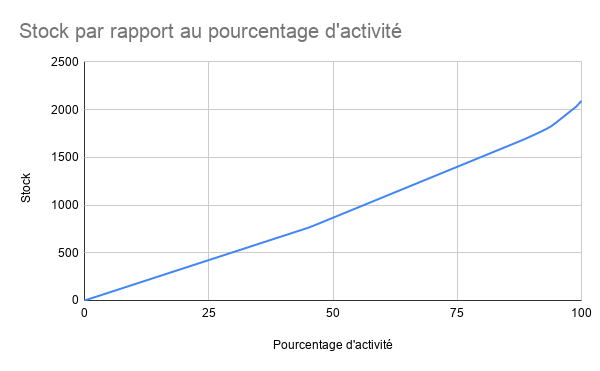
\includegraphics[width=1\textwidth]{img/Stock_Activite}
\caption{Stock en fonction du pourcentage d'activité}
\end{figure}
\end{center}

Nous pouvons remarquer qu'il y a 2 ruptures dans le tracé de cette fonction : 
\begin{itemize}
\item Une première rupture vers de 43\% de production maximale
\item Une deuxième rupture vers 93\% de production maximale
\end{itemize}

Pour connaître plus précisément ces positions de ruptures, nous avons tracé les courbes de tendances correspondant à chaque morceau. Nous avons obtenu les résultats suivants :

\begin{center}
\begin{figure}[H]
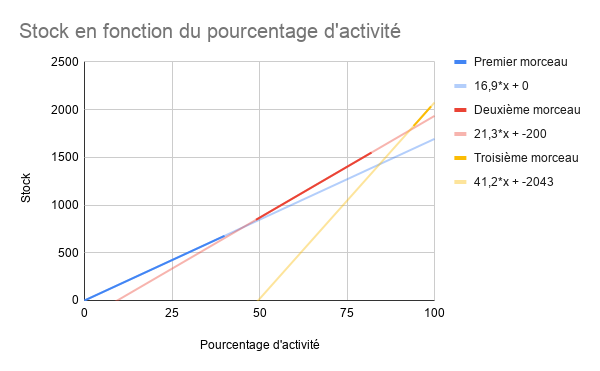
\includegraphics[width=1\textwidth]{img/Stock_Activite_tendance}
\caption{Stock en fonction du pourcentage d'activité avec courbes de tendance}
\end{figure}
\end{center}

Ces résultats nous permettre de déterminer les points de rupture :
\begin{itemize}
\item Premier point de rupture : intersection des 2 premières droites :\\
$16.9*P_{opt} = 21.3*P_{opt} - 200$ \\
Soit $P_{opt} = 45.5 \approx 45 $
\item Deuxième point de rupture : intersection des 2 dernières droites :\\
$41.2*P_{opt}-2043 = 21.3*P_{opt} - 200$ \\
Soit $P_{opt} = 92.6 \approx 93 $
\end{itemize}

Ces points sont importants puisque ce sont des points de rupture avant une grande augmentation des stocks. Le stock minimal est celui correspondant à une activité de 45\%, soit 762.2 unités. Cependant, il est difficile de demander à une entreprise de ne produire que 50\% de sa production maximale, c'est pourquoi l'entreprise pourrait choisir de produire 93\% de sa capacité maximale et avoir un stock de 1799.6 unités. 

\end{document}
\geometry{margin=2cm}
